\documentclass[
]{jss}

\usepackage[utf8]{inputenc}

\providecommand{\tightlist}{%
  \setlength{\itemsep}{0pt}\setlength{\parskip}{0pt}}

\author{
Hanne Oberman\\Utrecht University \And Johanna Munoz Avila\\University
Medical Center Utrecht \AND Valentijn de Jong\\University Medical
Center Utrecht \And Gerko Vink\\Utrecht University \AND Thomas
Debray\\University Medical Center Utrecht
}
\title{Imputation of Incomplete Multilevel Data with \pkg{mice}}

\Plainauthor{Hanne Oberman, Johanna Munoz Avila, Valentijn de
Jong, Gerko Vink, Thomas Debray}
\Plaintitle{Imputation of Incomplete Multilevel Data with mice}
\Shorttitle{Multilevel \pkg{mice}}


\Abstract{
Multilevel data is not spared the ubiquitous problem of missing
information. This is a tutorial paper on imputing incomplete multilevel
data with \pkg{mice}. Including methods for ignorable and non-ignorable
missingness. Footnotes in the current version show work in
progress/under construction. The last section is not part of the
manuscript, but purely for reminders.
}

\Keywords{missing
data, multilevel, clustering, \pkg{mice}, \proglang{R}}
\Plainkeywords{missing data, multilevel, clustering, mice, R}

%% publication information
%% \Volume{50}
%% \Issue{9}
%% \Month{June}
%% \Year{2012}
%% \Submitdate{}
%% \Acceptdate{2012-06-04}

\Address{
    Hanne Oberman\\
    Utrecht University\\
    Padualaan 14\\
3584 CH Utrecht\\
  E-mail: \email{h.i.oberman@uu.nl}\\
  URL: \url{https://hanneoberman.github.io/}\\~\\
          }

% Pandoc syntax highlighting

% Pandoc citation processing

\usepackage{graphicx}
\usepackage{mathtools}
\usepackage{ulem}

\usepackage{amsmath}

\begin{document}

\hypertarget{introduction}{%
\section{Introduction}\label{introduction}}

\hypertarget{multilevel-data}{%
\subsection{Multilevel data}\label{multilevel-data}}

\sout{Research into any field with a hierarchical or clustered nature of
observations may yield multilevel data. In the typical case, individuals
are nested within groups, but there are many different types of
multilevel data. In the medical field, clustering occurs at e.g., the
hospital or center level in registry data, or at the study-level in
meta-analyses (IPDMA). In the social sciences and official statistics we
can find clustering e.g.~at the country-level, or as imposed by a
multi-stage sampling design. For the sake of legibility, we will refer
to the grouping variable as `cluster', and the grouped variable as
`(sample) unit' throughout this paper. And, for reasons of brevity, we
only discuss clustering between units, not within units (e.g.,
timeseries or longitudinal data). Also, add that we'll only discuss two
levels, not more?}

In many contemporary data analysis efforts, some form of hierarchical or
clustered structure is recorded. Ignoring such structures may be harmful
to the inferences and can yield biased results. On the other hand,
analyzing such multilevel data requires specialized techniques that take
the clustered structure into account. Imagine a case where cross-level
interactions between unit-level variables and cluster-level variables
are present. The cluster to which a unit belongs may then influence the
unit-level observations - and vice versa - for each of the units that
make up the cluster \citep{hox17}. These relations can and should be
taken into account when developing analysis models for multilevel data
for the simple reason that groups of observations share some common
variance.

The variability due to clustering is often measured by means of the
intra-class coefficient (ICC). The ICC can be seen as the percentage of
variance that can be attributed to the cluster-level, where a high ICC
would indicate that a lot of variability is due to the cluster
structure. Multilevel models typically accommodate for this variability
by including separate intercepts for each cluster. Such fixed effects
relieve the restriction imposed by single-level models: equal group
means across clusters. Additionally, there may be random predictor
effects and/or random error terms (residual error variances), see e.g.
\citet{hox17} and \citet{jong21}.\footnote{Add that heterogeneity refers
  to variability within clusters.} There are many names for models that
take clustering into account. Some popular examples are `multilevel
models', `hierarchical models', `mixed effect models' and `random effect
models'.

\hypertarget{missing-data}{%
\subsection{Missing data}\label{missing-data}}

\begin{CodeChunk}
\begin{figure}

{\centering 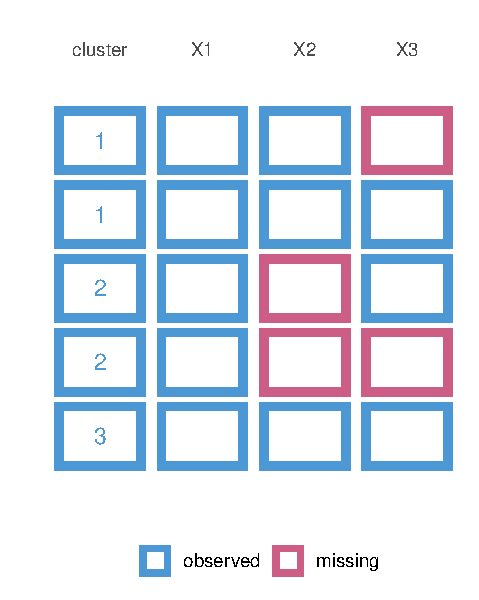
\includegraphics{Manuscript_files/figure-latex/patterns-1} 

}

\caption[Missingness in multilevel data]{Missingness in multilevel data}\label{fig:patterns}
\end{figure}
\end{CodeChunk}

The process of analyzing multilevel data is further complicated when not
all observations are observed. Just as with single level data,
missingness may occur at the unit level. But with multiple levels of
data comes the potential for clustered missingness. Missingness in
multilevel data can therefore be categorized into two general patterns:
systematic missingness and sporadic missingness, see \citet{resc13}. We
have visualized the difference between these types of missingness in
Figure 1. The figure shows an \(n \times p\) set
\(\mathbf{X} = X_1, \dots, X_p\), with \(n=5\) units and \(p=3\) columns
distributed over 3 clusters. Column \texttt{X1} is completely observed.
Column \texttt{X2} is systematically missing and column \texttt{X3} is
sporadically missing.\footnote{Explain why. GV: niet nodig}

Systematic missingness can be further subdivided into unobserved
constants (i.e., the same value within clusters) and non-measured random
variables (which may differ per unit within clusters). In Figure 1, the
former would imply that the unobserved values for units 3 and 4 on
column \texttt{X2} are identical. With the latter, the values would
differ. The optimal strategy for dealing with the missingness may
therefore depend on the observed missing data pattern. \footnote{add
  missing data mechanisms here? GV: No, patterns are different from
  mechanisms}

Ignoring the missingness in analyses can be extremely harmful to
inferences. Complete case analysis (i.e., excluding all units with one
or more missing entries) can introduce bias in statistical inference and
lowers statistical power. Instead, the missingness should be
accommodated \emph{before} or \emph{within} the analysis of scientific
interest. Especially the former is very generic and popular and is
widely known as imputation. Imputing (i.e., filling in) the missing
values separates the missing data problem from the scientific problem:
missing data are replaced by plausible values whereafter the completed
data is analysed as if it were completely observed. The \proglang{R}
package \pkg{mice} has become the de-facto standard for imputation by
chained equations, which iteratively solves the missingness on a
variable-by-variable basis. \pkg{mice} is known to yield valid
inferences under many different missing data circumstances
\citep{buur18}. In this paper, we'll discuss how to use \pkg{mice} in
the context of multilevel data, under varying missing data
mechanisms.\footnote{Discuss missingness mechanisms before this point,
  add references \citet{yuce08} and \citet{hox15}.}

\hypertarget{aim-of-this-paper}{%
\subsection{Aim of this paper}\label{aim-of-this-paper}}

This papers serves as a tutorial for imputing incomplete multilevel data
with \pkg{mice}. We provide practical guidelines and code snippets for
different missing data situations. For reasons of brevity, we focus on
imputation by chained equations\footnote{add that JOMO is available in
  \pkg{mice} as well?}. Other useful packages for incomplete multilevel
data include \pkg{mitml}, \pkg{miceadds}, and \pkg{mdmb}.\footnote{Rephrase:
  Some level of knowledge on multilevel models is assumed. We're
  providing an overview of implementations. It's up-to the reader to
  decide which multilevel strategy suits their data. So we won't go into
  detail for the different methods (and equations). Refer to
  \citet{meng94}, \citet{audi18}, and \citet{grun18}. This paper is just
  a software tutorial. We'll keep it practical.}

We structure this tutorial around three case studies:

\begin{itemize}
\item
  \texttt{mice::popmis} (simulated data on school kids, with MNAR/MAR
  mixture);
\item
  \texttt{metamisc::impact} (real IPD on traumatic brain injuries,
  without \texttt{NA}s);
\item
  \texttt{GJRM::hiv} (simulated patient data on HIV, without
  \texttt{NA}s)
\end{itemize}

For each case study we focus on a different aspect to illustrate how to
impute incomplete multilevel data. In the \texttt{mice::popmis} data, we
show the advantages of including the multilevel structure of the data
into the imputation model. In the \texttt{metamisc::impact} data we'll
show how to induce missingness and solve it in real-world data. In the
\texttt{GJRM::hiv} we provide novel methodology\footnote{not really, the
  methods exist already, but how to show that this is something new and
  exciting?} for imputing MNAR missingness according to the Heckman
model. For all case studies we discuss the nature of the incomplete
data, the imputation model(s), and evaluation of the imputed data.

\hypertarget{case-study-i-popularity}{%
\section{Case Study I: Popularity}\label{case-study-i-popularity}}

\texttt{popNCR} is a simulated dataset with pupils clustered in classes,
where the number of units \(n = 2000\), and the number of clusters
\(N = 100\), on 7 variables:

\begin{itemize}
\tightlist
\item
  \texttt{pupil} Pupil number within class,
\item
  \texttt{class} Class number,
\item
  \texttt{extrav} Pupil extraversion,
\item
  \texttt{sex} Pupil gender,
\item
  \texttt{texp} Teacher experience (years),
\item
  \texttt{popular} Pupil popularity,
\item
  \texttt{popteach} Teacher popularity.
\end{itemize}

\hypertarget{incomplete-data}{%
\subsubsection{Incomplete data}\label{incomplete-data}}

\begin{CodeChunk}
\begin{figure}

{\centering 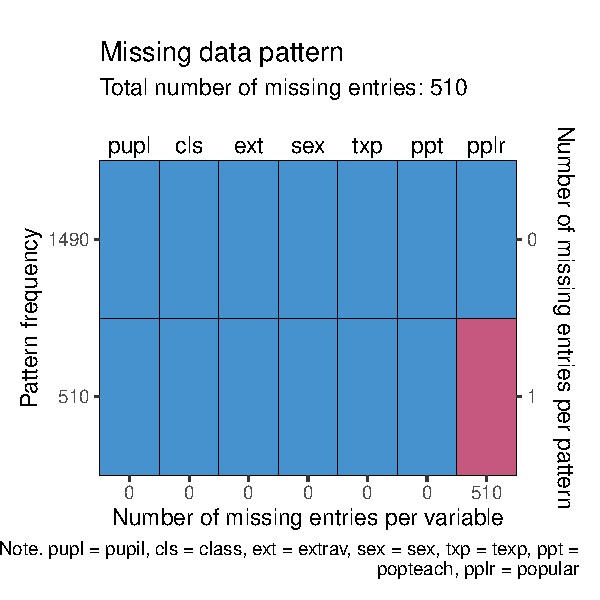
\includegraphics{Manuscript_files/figure-latex/pop_pat-1} 

}

\caption[Missing data pattern in the popularity data]{Missing data pattern in the popularity data}\label{fig:pop_pat}
\end{figure}
\end{CodeChunk}

The popularity data is created such that there are strong relations
between the incomplete variables and the clustering variable
\texttt{class}. We can express this using the intra-class correlation
(ICC). For \texttt{popular} the ICC is 0.33. For \texttt{popteach} it is
0.34. It would thus be wise to use multilevel modeling.

The missingness in this dataset is induced conform MAR and MNAR
mechanisms. The missing data pattern, Figure \ref{fig:pop_pat}, shows
that just one variable is incomplete \textbf{{[}the next part is not yet
updated to reflect this{]}}.

To develop the best imputation model, we need to know whether the
missingness in one variable depends on the observed values of other
variables. Visual inspection usually suffices. We'll highlight only two
variables to illustrate, but ideally one would inspect all relations.
The questions we'll ask are: `Does the missing data of \texttt{popular}
depend on \texttt{popteach}?' and `Does the missingness in teacher
popularity depend on pupil popularity?' We'll evaluate this by making a
histogram of \texttt{popteach} separately for the pupils with known
popularity and missing popularity, and the other way around.

In Figure \ref{fig:pop_dist} we see that the distribution for the
missing \texttt{popular} is further to the right than the distribution
for observed \texttt{popular}. This would indicate a right-tailed MAR
missingness. In fact, this is exactly what happens, because the
missingness in these data was created manually. Now, we've made it
observable by examining the relations between the missingness in popular
and the observed data in \texttt{popteach}. There is also a dependency
between the missingness in teacher popularity and pupil popularity. The
relation seems to be right-tailed as well.

\begin{CodeChunk}
\begin{figure}

{\centering 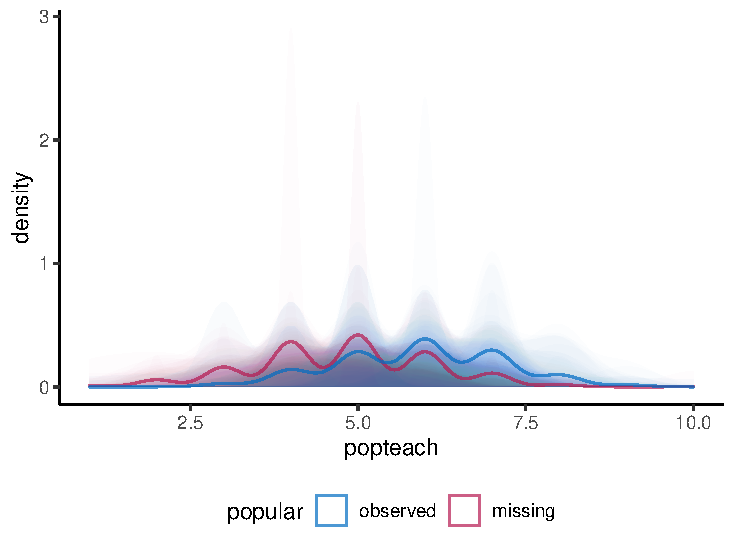
\includegraphics{Manuscript_files/figure-latex/pop_dist-1} 

}

\caption[Conditional distributions in the popularity data]{Conditional distributions in the popularity data}\label{fig:pop_dist}
\end{figure}
\end{CodeChunk}

\hypertarget{imputation-model}{%
\subsubsection{Imputation model}\label{imputation-model}}

The first imputation model that we'll use is likely to be invalid. In
this model, we ignore the multilevel structure of the data, despite the
high ICCs. This is purely to illustrate the effects of ignoring the
clustering in our imputation effort.

We'll use predictive mean matching to impute the continuous variables
and logistic regression to impute the binary variable \texttt{sex}. We
do not use the observation identifier \texttt{pupil} or cluster
identifier \texttt{class} as predictors to impute other variables.

\begin{CodeChunk}
\begin{CodeInput}
R> # dry run to get imputation parameters
R> ini <- mice(pop, maxit = 0)
R> 
R> # extract predictor matrix and adjust
R> pred <- ini$pred
R> pred[, c("class", "pupil")] <- 0
R> 
R> # impute the data, ignoring the cluster structure
R> imp_ignored <- mice(pop, maxit = 1, pred = pred, print = FALSE)
\end{CodeInput}
\end{CodeChunk}

\hypertarget{imputed-data}{%
\subsubsection{Imputed data}\label{imputed-data}}

\begin{CodeChunk}


\begin{center}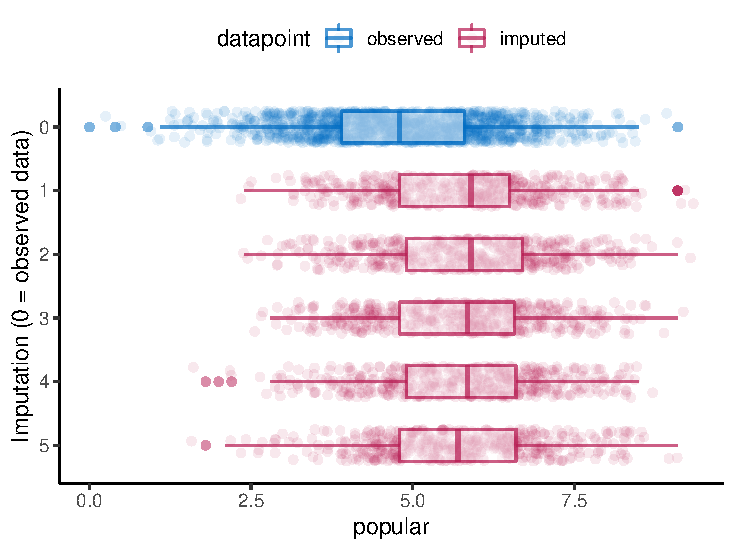
\includegraphics{Manuscript_files/figure-latex/pop_ignored_eval-1} \end{center}

\begin{CodeOutput}
      vars incomplete   ignored
1  popular  0.3280070 0.3338626
2 popteach  0.3414766 0.3414766
3     texp  1.0000000 1.0000000
\end{CodeOutput}
\end{CodeChunk}

As the original ICCs show, 100\% of the variance in \texttt{texp} can be
attributed to the clustering variable \texttt{class}. This tells us that
the multilevel structure of the data should be taken into account. If we
don't, we'll end up with incorrect imputations, biasing the effect of
the clusters towards zero.

We can also observe that the teacher experience increases slightly after
imputation. This is due to the MNAR missingness in \texttt{texp}. Higher
values for \texttt{texp} have a larger probability to be missing. This
may not a problem, however, if at least one pupil in each class has
teacher experience recorded, we can deductively impute the correct
(i.e.~true) value for every pupil in the class.

\hypertarget{imputation-model-1}{%
\subsubsection{Imputation model}\label{imputation-model-1}}

We'll now use \texttt{class} as a predictor to impute all other
variables. This is still not recommended practice, since it only works
under certain circumstances and results may be biased. But at least, it
includes some multilevel aspect. Colloquially, this is `multilevel
imputation for dummies'.

\begin{CodeChunk}
\begin{CodeInput}
R> # adjust the predictor matrix
R> pred <- ini$pred 
R> pred[, "pupil"] <- 0
R> 
R> # impute the data, cluster as predictor
R> imp_predictor <- mice(pop, maxit = 1, pred = pred, print = FALSE)
\end{CodeInput}
\end{CodeChunk}

\hypertarget{imputed-data-1}{%
\subsubsection{Imputed data}\label{imputed-data-1}}

\begin{CodeChunk}


\begin{center}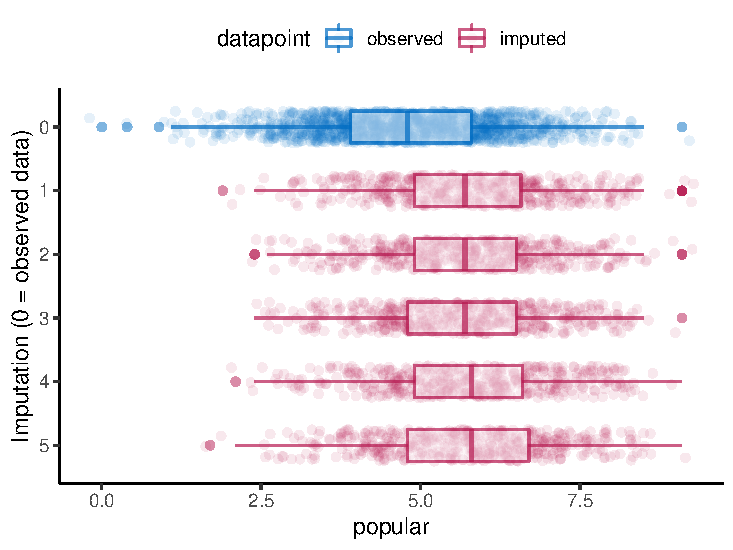
\includegraphics{Manuscript_files/figure-latex/pop_predictor_eval-1} \end{center}

\begin{CodeOutput}
      vars incomplete   ignored predictor
1  popular  0.3280070 0.3338626 0.3871020
2 popteach  0.3414766 0.3414766 0.3414766
3     texp  1.0000000 1.0000000 1.0000000
\end{CodeOutput}
\end{CodeChunk}

Now, we can clearly see that the imputed values of \texttt{texp} are
higher than the observed values, which is in line with right-tailed
MNAR.

The ICCs are way more in line with the ICCs in the incomplete data. But
this is a quick and dirty way of imputing multilevel data. We
\emph{should} be using a multilevel model.

\hypertarget{imputation-model-2}{%
\subsubsection{Imputation model}\label{imputation-model-2}}

To include\ldots{}

\begin{CodeChunk}
\begin{CodeInput}
R> pred <- ini$pred
R> pred["popular", ] <- c(0, -2, 2, 2, 2, 0, 2) 
R> #-2 for the cluster variable, 2 for random effects
R> meth <- ini$meth
R> meth <- c("", "", "", "", "", "2l.norm", "")
R> imp_norm_2l <-
+   mice(
+     pop %>% mutate(class = as.integer(class)),
+     pred = pred,
+     meth = meth,
+     maxit = 1,
+     print = FALSE
+   )
\end{CodeInput}
\end{CodeChunk}

\begin{CodeChunk}
\begin{CodeInput}
R> # plot(imp_norm)
R> plot_box(imp_norm_2l, x = "popular", strip = TRUE)
\end{CodeInput}


\begin{center}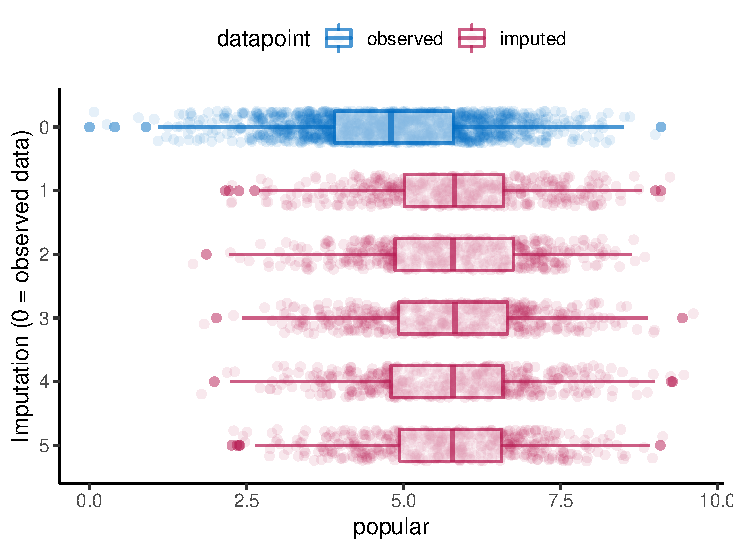
\includegraphics{Manuscript_files/figure-latex/pop_norm_eval-1} \end{center}

\begin{CodeInput}
R> ICCs <- ICCs %>% mutate(
+            norm = c(icc(popular ~ as.factor(class), complete(imp_norm_2l)), 
+                     icc(popteach ~ as.factor(class), complete(imp_norm_2l)), 
+                     icc(texp ~ as.factor(class), complete(imp_norm_2l)))
+            )
R> ICCs
\end{CodeInput}
\begin{CodeOutput}
      vars incomplete   ignored predictor      norm
1  popular  0.3280070 0.3338626 0.3871020 0.3612830
2 popteach  0.3414766 0.3414766 0.3414766 0.3414766
3     texp  1.0000000 1.0000000 1.0000000 1.0000000
\end{CodeOutput}
\end{CodeChunk}

\begin{CodeChunk}
\begin{CodeInput}
R> pred["popular", ] <- c(0, -2, 2, 2, 1, 0, 2)
R> meth <- c("", "", "", "", "", "2l.pan", "")
R> imp_pan_2l <-
+   mice(
+     pop %>% mutate(class = as.integer(class)),
+     pred = pred,
+     meth = meth,
+     maxit = 1,
+     print = FALSE
+   )
\end{CodeInput}
\end{CodeChunk}

\begin{CodeChunk}
\begin{CodeInput}
R> # plot(imp_pan)
R> plot_box(imp_pan_2l, x = "popular", strip = TRUE)
\end{CodeInput}


\begin{center}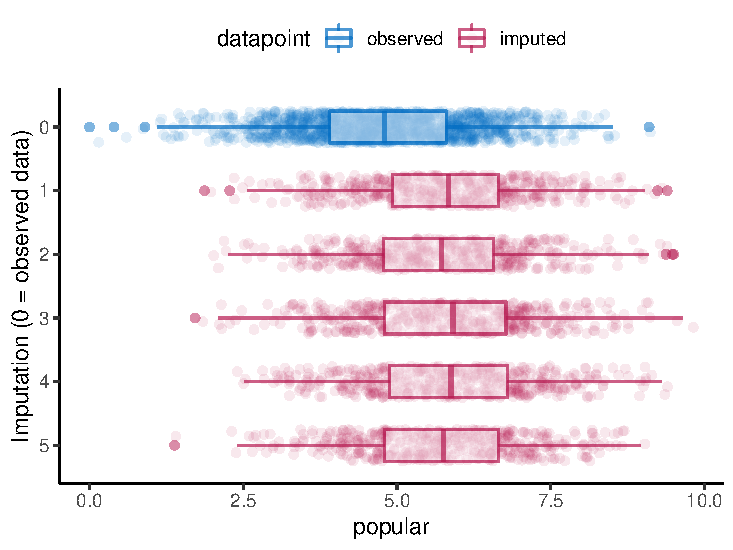
\includegraphics{Manuscript_files/figure-latex/pop_pan_eval-1} \end{center}

\begin{CodeInput}
R> ICCs <- ICCs %>% mutate(
+            pan = c(icc(popular ~ as.factor(class), complete(imp_pan_2l)), 
+                     icc(popteach ~ as.factor(class), complete(imp_pan_2l)), 
+                     icc(texp ~ as.factor(class), complete(imp_pan_2l)))
+            )
R> ICCs
\end{CodeInput}
\begin{CodeOutput}
      vars incomplete   ignored predictor      norm       pan
1  popular  0.3280070 0.3338626 0.3871020 0.3612830 0.3745108
2 popteach  0.3414766 0.3414766 0.3414766 0.3414766 0.3414766
3     texp  1.0000000 1.0000000 1.0000000 1.0000000 1.0000000
\end{CodeOutput}
\end{CodeChunk}

\hypertarget{case-study-ii-impact}{%
\section{Case study II: IMPACT}\label{case-study-ii-impact}}

\texttt{impact} is traumatic brain injury data with patients,
\(n = 11022\), clustered in studies, \(N = 15\). With the following 11
variables:

\begin{itemize}
\tightlist
\item
  \texttt{name} Name of the study,
\item
  \texttt{type} Type of study (RCT: randomized controlled trial, OBS:
  observational cohort),
\item
  \texttt{age} Age of the patient,
\item
  \texttt{motor\_score} Glasgow Coma Scale motor score,
\item
  \texttt{pupil} Pupillary reactivity,
\item
  \texttt{ct} Marshall Computerized Tomography classification,
\item
  \texttt{hypox} Hypoxia (0=no, 1=yes),
\item
  \texttt{hypots} Hypotension (0=no, 1=yes),
\item
  \texttt{tsah} Traumatic subarachnoid hemorrhage (0=no, 1=yes),
\item
  \texttt{edh} Epidural hematoma (0=no, 1=yes),
\item
  \texttt{mort} 6-month mortality (0=alive, 1=dead).
\end{itemize}

The data is already imputed (Steyerberg et al, 2008), so we'll induce
missingness ourselves. For example, MAR missingness varying by
cluster.\footnote{Observed data pattern should differ per cluster. So,
  in cluster 1, the missingness would depend on age, but not in cluster
  two. Split the dataframe and run \texttt{ampute()} on each cluster.}

\hypertarget{case-study-iii-hiv}{%
\section{Case study III: HIV}\label{case-study-iii-hiv}}

Toy example from
\href{https://github.com/johamunoz/Heckman-IPDMA/blob/main/Toy_example.R}{Heckman
Github repo}. We will use the following variables:

\begin{itemize}
\tightlist
\item
  \texttt{region} Cluster variable,
\item
  \texttt{hiv} HIV diagnosis (0=no, 1=yes),
\item
  \texttt{age} Age of the patient,
\item
  \texttt{marital} Marital status,
\item
  \texttt{condom} Condom use during last intercourse,
\item
  \texttt{smoke} Smoker (levels).
\end{itemize}

\begin{CodeChunk}


\begin{center}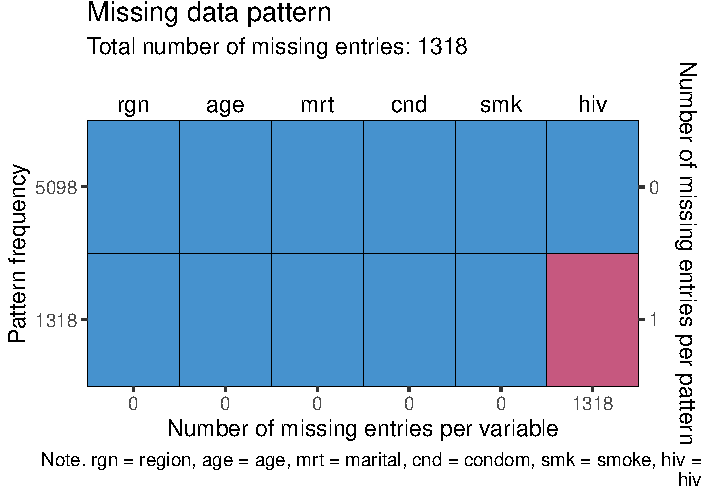
\includegraphics{Manuscript_files/figure-latex/hiv-1} \end{center}

\end{CodeChunk}

\hypertarget{discussion}{%
\section{Discussion}\label{discussion}}

\begin{itemize}
\item
  JOMO in \pkg{mice} -\textgreater{} on the side for now
\item
  Additional levels of clustering
\item
  More complex data types: timeseries and polynomial relationship in the
  clustering.
\end{itemize}

\hypertarget{think-about}{%
\section{Think about}\label{think-about}}

\begin{itemize}
\item
  Adding some kind of help function to mice that suggests a suitable
  predictor matrix to the user, given a certain analysis model.
\item
  Adding a \texttt{multilevel\_ampute()} wrapper function in mice.
\item
  Exporting \texttt{mids} objects to other packages like \texttt{lme4}
  or \texttt{coxme}?
\item
  Adding a ICC=0 dataset to show that even if there is no clustering it
  doesn't hurt.
\end{itemize}

\renewcommand\refname{References}
\bibliography{../References/multilevelmice.bib}


\end{document}
